\section{Heavy-tailed runs}\label{sec:heavy}

In this section the walk remembers the time since its last switch. The steps form
maximal runs whose directions alternate. The first run has length $D$, and the later
runs have i.i.d.\ lengths $\xi_1,\xi_2,\dots$ distributed as $\xi$, where
$\bar F(k)=\Prob(\xi\ge k)=k^{-\alpha}$ for $k\ge1$ and some $\alpha>0$. So
$p_k=\Prob(\xi=k)=k^{-\alpha}-(k+1)^{-\alpha}>0$ for every $k\ge1$. The first direction
is fair, and $D$, $(\xi_i)$ and the first direction are independent. With a fresh start
$D$ has the law of $\xi$. For $\alpha>1$ the stationary start is
$\Prob(D=d)=\bar F(d)/\mu$, where $\mu=\E\xi=\zeta(\alpha)$. This law is stationary,
since the number of steps left in the current run (counting the current one) is a Markov
chain that moves from $k\ge2$ to $k-1$ and from $1$ to a fresh copy of $\xi$, and
$\bar F(k)=\bar F(k+1)+p_k\bar F(1)$ makes $\bar F(k)/\mu$ invariant. We define $A_n$,
$C_n$ and $E_n$ as in Section~\ref{sec:intro}, put $R_n=E_n/C_n$, and write $\Prob_+$
for the law given that the first run is $+$.

\begin{proposition}[the edge]\label{prop:edge}
For every law of $D$, $E_n=\frac12\Prob(D\ge n)$. With a fresh start
$E_n=\frac12n^{-\alpha}$. With the stationary start
$E_n=\zeta(\alpha,n)/(2\zeta(\alpha))=n^{1-\alpha}(1+\theta_n(\alpha-1)/n)/(2(\alpha-1)\zeta(\alpha))$
for some $\theta_n\in[0,1]$, where $\zeta(\alpha,n)=\sum_{k\ge n}k^{-\alpha}$ is the
Hurwitz zeta function.
\end{proposition}

\begin{proof}
All $n$ steps are $+1$ exactly when the first direction is $+$ and $D\ge n$. Hence
$E_n=\frac12\Prob(D\ge n)$, and $\Prob(\xi\ge n)=n^{-\alpha}$. For the stationary start
$\Prob(D\ge n)=\zeta(\alpha,n)/\zeta(\alpha)$. Since $x^{-\alpha}$ is decreasing,
$\int_n^\infty x^{-\alpha}dx\le\zeta(\alpha,n)\le n^{-\alpha}+\int_n^\infty x^{-\alpha}dx$,
and the integral equals $n^{1-\alpha}/(\alpha-1)$.
\end{proof}

So the edge only sees the first run, while the center depends on all the runs. Let
$\tau_m=\xi_1+\dots+\xi_m$ with $\tau_0=0$, $u_m(k)=\Prob(\tau_m=k)$ and
$q_m(k)=\Prob(\tau_{m-1}<k\le\tau_m)=\sum_{j\ge1}\bar F(j)u_{m-1}(k-j)$ for $m,k\ge1$.
For the delayed versions let $D$ be independent of $(\xi_i)$, and put
$u^D_m(k)=\Prob(D+\tau_{m-1}=k)$, $q^D_1(k)=\Prob(D\ge k)$ and
$q^D_m(k)=\Prob(D+\tau_{m-2}<k\le D+\tau_{m-1})$ for $m\ge2$. For the stationary start
$u^D_m(k)=\sum_d\frac{\bar F(d)}{\mu}u_{m-1}(k-d)=q_m(k)/\mu$.

The $+$ runs and the $-$ runs form 2 independent renewal processes. The walk is in bin
$a$ at time $n$ exactly when one of them sits at its level and the other is inside a run
that covers its level.

\begin{proposition}[two renewal processes]\label{prop:tworenewal}
Let $D$ have any law on $\{1,2,\dots\}$. For $a+b=n$ with $a,b\ge1$,
\[
 \Prob_+(A_n=a)=\sum_{m\ge1}\Bigl[u_m(b)\,q^D_{m+1}(a)+u^D_m(a)\,q_m(b)\Bigr],
\]
and $\Prob_+(A_n=n)=\Prob(D\ge n)$. In particular, for even $n$,
$C_n=\sum_{m\ge1}[u_m(h)q^D_{m+1}(h)+u^D_m(h)q_m(h)]$. For the fresh start this is
$C_n=\sum_mu_m(h)[q_m(h)+q_{m+1}(h)]$.
\end{proposition}

\begin{proof}
Let the $+$ runs have lengths $D,\xi^+_2,\xi^+_3,\dots$ and the $-$ runs
$\xi^-_1,\xi^-_2,\dots$, and let $s^\pm_j$ be the sum of the first $j$ lengths of each
sign, with $s^\pm_0=0$. So $s^+_j$ has law $u^D_j$ and $s^-_j$ has law $u_j$, and the 2
sequences are independent. The $j$-th $+$ run covers the steps in
$(s^+_{j-1}+s^-_{j-1},\,s^+_j+s^-_{j-1}]$, and the $j$-th $-$ run covers
$(s^+_j+s^-_{j-1},\,s^+_j+s^-_j]$. If step $n=a+b$ is in the first run then $A_n=n$,
which happens exactly when $D\ge n$. If it is in the $j$-th $+$ run with $j\ge2$, then
$A_n=n-s^-_{j-1}$, so $A_n=a$ means $s^-_{j-1}=b$ and $s^+_{j-1}<a\le s^+_j$, which has
probability $u_{j-1}(b)q^D_j(a)$. If it is in the $j$-th $-$ run, then $A_n=s^+_j$, so
$A_n=a$ means $s^+_j=a$ and $s^-_{j-1}<b\le s^-_j$, which has probability
$u^D_j(a)q_j(b)$. Summing over these disjoint cases, with $m=j-1$ in the first and $m=j$
in the second, gives the formula. For even $n$ the symmetry gives
$C_n=\frac12[\Prob_+(A_n=h)+\Prob_+(A_n=n-h)]=\Prob_+(A_n=h)$.
\end{proof}

This identity is the coefficient form of the double transform of Godr\`eche and
Luck~\cite[Section~7]{godrecheluck2001} for the occupation time of an alternating
renewal process.

\begin{lemma}[stable and local limits]\label{lem:stable}
Let $1<\alpha<2$ and $a_m=m^{1/\alpha}$. Put
$K_\alpha=\Gamma(2-\alpha)/(\alpha-1)=-\Gamma(1-\alpha)>0$ and
$\sigma_\alpha=2K_\alpha\lvert\cos\frac{\pi\alpha}2\rvert$.
\begin{enumerate}[(i)]
\item $\E e^{i\theta\xi}=1+i\mu\theta+K_\alpha(-i\theta)^\alpha+O(\theta^2)$ as
$\theta\to0$, with the principal branch.
\item $(\tau_m-m\mu)/a_m$ converges in law to a variable $G$ with
$\E e^{-sG}=e^{K_\alpha s^\alpha}$ for $s\ge0$ and
$\E e^{i\theta G}=\exp(K_\alpha(-i\theta)^\alpha)$. The law of $G$ is totally skewed to
the right and has a bounded, uniformly continuous density $g$ with $g(z)\to0$ as
$\lvert z\rvert\to\infty$.
\item (Gnedenko) $\sup_k\lvert a_mu_m(k)-g((k-m\mu)/a_m)\rvert\to0$, and
$\bar u:=\sup_{m\ge1}\sup_ka_mu_m(k)<\infty$.
\item If $G'$ is an independent copy of $G$, then $G-G'$ is symmetric $\alpha$-stable
with $\E e^{i\theta(G-G')}=e^{-\sigma_\alpha\lvert \theta\rvert^\alpha}$, and
$I_\alpha:=\int_{\mathbb R}g(z)^2\,dz=\Gamma(1+1/\alpha)/(\pi\sigma_\alpha^{1/\alpha})$.
\end{enumerate}
\end{lemma}

\begin{proof}
(i) Summation by parts gives $1-\E x^\xi=(1-x)\sum_{k\ge1}\bar F(k)x^{k-1}$ for
$\lvert x\rvert\le1$. With $x=e^{-u}$ and
$\mathrm{Li}_\alpha(w)=\sum_{k\ge1}k^{-\alpha}w^k$ this is
$1-\E e^{-u\xi}=(e^u-1)\mathrm{Li}_\alpha(e^{-u})$. For $\operatorname{Re}u\ge0$ and
$0<\lvert u\rvert<2\pi$, \cite[25.12.12]{dlmf} gives
$\mathrm{Li}_\alpha(e^{-u})=\Gamma(1-\alpha)u^{\alpha-1}+\zeta(\alpha)+O(\lvert u\rvert)$.
So $1-\E e^{-u\xi}=\mu u+\Gamma(1-\alpha)u^\alpha+O(\lvert u\rvert^2)$, and $u=-i\theta$
gives (i). (ii) By (i),
$e^{-i\mu t}\E e^{it\xi}=1+K_\alpha(-i\theta)^\alpha/m+O(\theta^2m^{-2/\alpha})$ for
$t=\theta/a_m$. As $2/\alpha>1$, the characteristic function of $(\tau_m-m\mu)/a_m$
tends to $\exp(K_\alpha(-i\theta)^\alpha)$, whose modulus
$\exp(-\frac12\sigma_\alpha\lvert\theta\rvert^\alpha)$ is integrable. L\'evy's
continuity theorem, Fourier inversion and the Riemann--Lebesgue lemma give $G$ and $g$
(the domain of attraction also follows from \cite[Theorem~XVII.5.2]{feller1971}). For
real $s>0$, the expansion of $1-\E e^{-u\xi}$ above with $u=s/a_m$ gives
$\E e^{-s(\tau_m-m\mu)/a_m}\to e^{K_\alpha s^\alpha}$ in the same way,
and with $2s$ in place of $s$ this gives uniform integrability, so
$\E e^{-sG}=e^{K_\alpha s^\alpha}$. (iii) Every $p_k$ is positive, so $\xi$ has maximal
span 1, and Gnedenko's local limit theorem~\cite[Chapter~4]{ibragimovlinnik1971}
gives the limit. Then
$a_mu_m(k)\le\lVert g\rVert_\infty+1$ for large $m$ and $a_mu_m(k)\le a_m$ for the
others, so $\bar u<\infty$. (iv) The function
$\lvert\E e^{i\theta G}\rvert^2=e^{-\sigma_\alpha\lvert\theta\rvert^\alpha}$ is the
characteristic function of $G-G'$, and Plancherel's theorem gives
$I_\alpha=\frac1{2\pi}\int e^{-\sigma_\alpha\lvert\theta\rvert^\alpha}d\theta$, which is
$\Gamma(1+1/\alpha)/(\pi\sigma_\alpha^{1/\alpha})$.
\end{proof}

\begin{theorem}[the center for $1<\alpha<2$]\label{thm:center}
Let $1<\alpha<2$ and let $D$ be any a.s.\ finite first run, in particular either start.
As $n\to\infty$ over even $n$,
\[
 C_n\sim2I_\alpha\Bigl(\frac{\mu}{h}\Bigr)^{1/\alpha}
 =\frac{2\Gamma(1+1/\alpha)}{\pi}\Bigl(\frac{\mu}{K_\alpha\lvert\cos(\pi
 \alpha/2)\rvert\,n}\Bigr)^{1/\alpha}.
\]
\end{theorem}

Both kinds of runs must fill about $h$ steps, which takes about $h/\mu$ runs of each
kind. Each renewal process is then within about $n^{1/\alpha}$ of its mean, so the 2
meet at a given level with probability of order $n^{-1/\alpha}$. In the proof (Appendix~\ref{app:heavy}) we split
the sum in Proposition~\ref{prop:tworenewal} by the number $m$ of runs. With
$b_h=(h/\mu)^{1/\alpha}$, the terms with $\lvert m\mu-h\rvert\le Mb_h$ form a Riemann
sum for $2b_h^{-1}\int_{-M}^Mg^2$ by Lemma~\ref{lem:stable}(iii). The terms with
$m\le h/(4\mu)$ add up to $O(h^{-\alpha})=o(b_h^{-1})$, since a large sum of few runs is
most likely made by one long run. The others add up to
$O(b_h^{-1})\Prob(\lvert G\rvert\ge M-1)+o(b_h^{-1})$, and we let $M\to\infty$.

With a stationary start the first run covers all $n$ steps with probability of order
$n^{1-\alpha}$, and this is comparable with $C_n$ when $1-\alpha=-1/\alpha$, that is
$\alpha^2-\alpha-1=0$.

\begin{corollary}[the golden-ratio exponent]\label{cor:golden}
Let $1<\alpha<2$ and $e(\alpha)=1-\alpha+1/\alpha$. If
$\Prob(D\ge n)\sim c_Dn^{-\beta_D}$ with $c_D,\beta_D>0$, then
$R_n\sim c_Dn^{1/\alpha-\beta_D}/(4I_\alpha(2\mu)^{1/\alpha})$. In particular
$R_n\sim C(\alpha)n^{e(\alpha)}$ for the stationary start and
$R_n\sim C_{\rm fr}(\alpha)n^{e(\alpha)-1}$ for the fresh start, where
\[
 C(\alpha)=\frac{\pi\bigl(K_\alpha\lvert\cos\frac{\pi\alpha}2\rvert
 \bigr)^{1/\alpha}}{4(\alpha-1)\Gamma(1+\frac1\alpha)\,
 \zeta(\alpha)^{1+1/\alpha}},\qquad
 C_{\rm fr}(\alpha)=(\alpha-1)\zeta(\alpha)\,C(\alpha).
\]
Since $e(\alpha)>0$ exactly when $\alpha<\varphi$, with a stationary start the ends win
for all large $n$ if $\alpha<\varphi$, and the center wins if $\alpha>\varphi$. At
$\alpha=\varphi$,
\[
 R_n\to C(\varphi)=\frac{\pi\varphi\bigl(\varphi\,\Gamma(\varphi^{-2})\lvert
 \cos\frac{\pi\varphi}2\rvert\bigr)^{1/\varphi}}{4\,\Gamma(\varphi)\,
 \zeta(\varphi)^{\varphi}}=0.7761317206\ldots,
\]
so the center still wins by the factor $1/C(\varphi)=1.2884$. With a fresh start
$e(\alpha)-1<0$, and the center wins for every $1<\alpha<2$.
\end{corollary}

\begin{proof}
By Proposition~\ref{prop:edge} and Theorem~\ref{thm:center}, with $h=n/2$, we have
$R_n=\Prob(D\ge n)/(2C_n)$, and this is asymptotic to
$c_Dn^{-\beta_D}/(4I_\alpha(2\mu/n)^{1/\alpha})$, which is the general formula. By
Lemma~\ref{lem:stable}(iv),
$4I_\alpha(2\mu)^{1/\alpha}=4\Gamma(1+\frac1\alpha)\mu^{1/\alpha}/(\pi(K_\alpha\lvert\cos\frac{\pi\alpha}2\rvert)^{1/\alpha})$.
The fresh start has $c_D=1$ and $\beta_D=\alpha$, which gives $C_{\rm fr}(\alpha)$. By
Proposition~\ref{prop:edge} the stationary start has $c_D=1/((\alpha-1)\mu)$ and
$\beta_D=\alpha-1$, which gives $C(\alpha)$. Next,
$e(\alpha)=-(\alpha^2-\alpha-1)/\alpha$, and $\varphi$ is the positive root of
$\alpha^2-\alpha-1$. At $\alpha=\varphi$ we have $\alpha-1=1/\varphi$,
$1+1/\alpha=\varphi$ and $2-\alpha=\varphi^{-2}$. So
$K_\varphi=\varphi\,\Gamma(\varphi^{-2})$, and substituting these into $C(\alpha)$ gives
the closed form.
\end{proof}

Corollary~\ref{cor:golden} is the lattice form, with its constant, of the heuristic of
Wang, Li and H\"anggi~\cite[Section~2.1]{wlh2016}. The golden ratio also appears for
the elephant walk, as the log-concavity threshold $1/\varphi$
of~\cite[Proposition~2.2]{glrs2025}, but we know of no connection between the 2. The
approach to $C(\varphi)$ is slow. At $\alpha=\varphi$ we have $R_{10^5}/C(\varphi)=0.938$,
and $R_n$ increases on the computed grid
(Table~\ref{tab:heavy} and Figure~\ref{fig:heavy}).

\begin{table}[t]
\centering\small
\setlength{\tabcolsep}{5pt}
\begin{tabular}{@{}lrlllll@{}}
\toprule
$\alpha$ & $e(\alpha)$ & $C(\alpha)$ & $C_{\rm fr}(\alpha)$ & $R_{1600}$ & $R_{10^4}$ & $R_{10^5}$\\
\midrule
$1.3$ & $+0.469231$ & $0.422717$ & $0.498631$ & $17.7593$ $[1.3180]$ & $38.7537$ $[1.2171]$ & $106.149$ $[1.1317]$\\
$1.5$ & $+0.166667$ & $0.647971$ & $0.846371$ & $2.14409$ $[0.9675]$ & $2.9528$ $[0.9818]$ & $4.37642$ $[0.9914]$\\
$\varphi$ & $0$ & $0.776132$ & $1.073675$ & $0.661763$ $[0.8526]$ & $0.697331$ $[0.8985]$ & $0.727689$ $[0.9376]$\\
$5/3$ & $-1/15$ & $0.835101$ & $1.182237$ & $0.411815$ $[0.8064]$ & $0.389307$ $[0.8614]$ & $0.352822$ $[0.9102]$\\
$1.7$ & $-0.111765$ & $0.880046$ & $1.265508$ & $0.298369$ $[0.7733]$ & $0.262005$ $[0.8334]$ & $0.215839$ $[0.8881]$\\
$1.9$ & $-0.373684$ & $1.438986$ & $2.266075$ & $0.0449706$ $[0.4923]$ & $0.0256505$ $[0.5569]$ & $0.0121612$ $[0.6242]$\\
\bottomrule
\end{tabular}
\caption{Constants of Corollary~\ref{cor:golden} and exact values of $R_n=E_n/C_n$ for
the stationary start, with $R_n/(C(\alpha)n^{e(\alpha)})$ in brackets.}
\label{tab:heavy}
\end{table}

\begin{figure}[t]
\centering
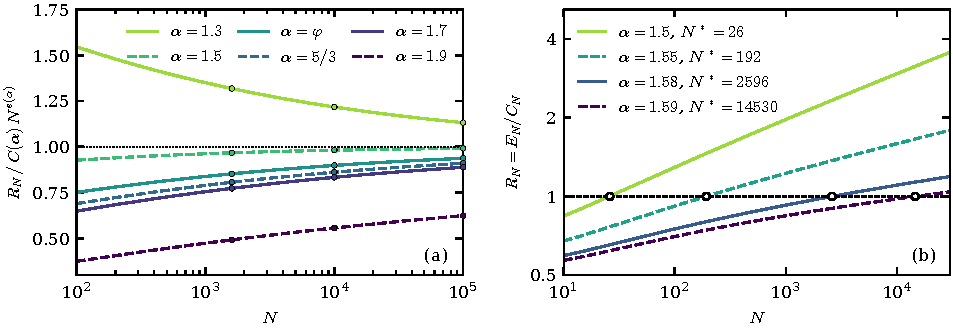
\includegraphics{figures/heavy}
\caption{Alternating runs with a stationary start. (a) $R_n/(C(\alpha)n^{e(\alpha)})$ for
even $n$ from 100 to $10^5$, with the entries of Table~\ref{tab:heavy} as dots. (b)
$R_n$ for $\alpha=1.5,1.55,1.58,1.59$ below $\varphi$. Each curve crosses 1 once on
$10\le n\le3\cdot10^4$, at $n^*(\alpha)$ (circles).}
\label{fig:heavy}
\end{figure}

\begin{table}[t]
\centering\small
\setlength{\tabcolsep}{4pt}
\begin{tabular}{@{}lllll@{}}
\toprule
$\alpha$ & start & center $C_n$ & ratio $R_n$ & status\\
\midrule
$\alpha>2$ & stationary & $\sim\sqrt{2\mu/(\pi vn)}$ & $\sim C_2(\alpha)n^{3/2-\alpha}$ & same argument, omitted\\
$\alpha=2$ & stationary & $\sim\sqrt{2\mu/(\pi n\log n)}$ & $\sim\sqrt{\pi\log n/(8\zeta(2)^3n)}$ & same argument, omitted\\
$1<\alpha<2$ & fresh & $\sim2I_\alpha(\mu/h)^{1/\alpha}$ & $\sim C_{\rm fr}(\alpha)n^{e(\alpha)-1}\to0$ & Corollary~\ref{cor:golden}\\
$\alpha=1$ & fresh & $\approx2/(\pi^2\tilde m_h)$ & $\approx\pi^2\tilde m_h/(8h)\sim\pi^2/(8\log n)$ & heuristic\\
$0<\alpha<1$ & fresh & $\sim\frac2\pi\tan\frac{\pi\alpha}2\cdot\frac1n$ & $\sim\frac{\pi}{4\tan(\pi\alpha/2)}\,n^{1-\alpha}\to\infty$ & proof omitted\\
\bottomrule
\end{tabular}
\caption{Outcomes of Remark~\ref{rem:other}. The center wins when $R_n\to0$ and the ends
win when $R_n\to\infty$.}
\label{tab:outcomes}
\end{table}

\begin{remark}[other exponents]\label{rem:other}
Table~\ref{tab:outcomes} collects the cases that Corollary~\ref{cor:golden} leaves out.
For $\alpha>2$ let $v=\Var\xi=2\zeta(\alpha-1)-\zeta(\alpha)-\zeta(\alpha)^2$ and
$C_2(\alpha)=\sqrt{\pi v/(2\mu)}/(2(\alpha-1)\mu)$. The proof of
Theorem~\ref{thm:center} works with the Gaussian local limit theorem and
$a_m=\sqrt{vm}$, and for $\alpha=2$ with the norming $a_m\sim\sqrt{m\log m}$
of~\cite[Theorem~XVII.5.3 and eq.~(XVII.5.23)]{feller1971}. In these 2 rows the center
formula holds for every a.s.\ finite first run, so a fresh start also gives $R_n\to0$.
For $\alpha=1$ the same proof with a skewed Cauchy limit and the centering
$m(H_{m+1}-1)$ suggests the row of the table, where $\tilde m_h$ solves
$m(H_{m+1}-1)=h$. For $0<\alpha<1$ only the fresh start makes
sense, and $\frac2\pi\tan\frac{\pi\alpha}2$ is the density at $\frac12$ of Lamperti's
occupation-time law~\cite{lamperti1958,godrecheluck2001}. Here the proof splits the sum
in Proposition~\ref{prop:tworenewal} on the scale of $\log m$ and uses the moments of a
positive stable law~\cite[Theorem~2.6.3]{zolotarev1986} and the series for its
density~\cite[Lemma~XVII.6.1]{feller1971}. We omit the details for $\alpha\ge2$ and
$0<\alpha<1$. So with a fresh start the threshold is $\alpha=1$.
\end{remark}

\begin{remark}[crossover sizes and heat conduction]\label{rem:crossover}
For $\alpha<\varphi$ and a stationary start the crossover is late when $\alpha$ is close
to $\varphi$. For $\alpha=1.5,1.55,1.58,1.59$ and every even $n$ in $[10,3\cdot10^4]$,
$R_n-1$ changes sign once, at $n^*(\alpha)=26,192,2596,14530$. Heuristically, $C(\alpha)n^{e(\alpha)}=1$
gives $\log n^*(\alpha)=0.1834/(\varphi-\alpha)+O(1)$ as $\alpha\uparrow\varphi$. At the
value $\alpha=5/3$ of L\'evy-walk models of heat conduction~\cite{dsd2013,zdk2015},
$R_n\sim C(5/3)n^{-1/15}$ with $C(5/3)=0.8351$.
\end{remark}

\begin{remark}[aging]\label{rem:aging}
Let the walk take a fair first step and then switch direction at step $k\ge2$ with
probability $c/k$, where $0<c<2$. Then $A_n/n$ converges in law to
$\mathrm{Beta}(c,c)$~\cite[Example~1.1 and Theorem~1.4]{ds2007} (their chain is this
walk for $c\le1$), \cite[Theorem~1]{ev2018}, and the limit is uniform exactly when
$c=1$~\cite[Remark~2]{ev2018}. At finite $n$ the first step matters. Let $\Prob_+$ be
the law given that the first step is $+1$, and let $X_n$ be the last step. At $c=1$
induction on $n\ge2$ gives $\Prob_+(A_n=s,\,X_n=+1)=\frac{s-1}{n(n-1)}$ and
$\Prob_+(A_n=s,\,X_n=-1)=\frac{n-s}{n(n-1)}$ for $1\le s\le n$, so $A_n$ is uniform on
$\{1,\dots,n\}$ (after a shift of one step this is the exercise
in~\cite[footnote~1 on p.~6]{evw2020}). Compared with no switch, a switch at time $t$
multiplies the probability of a path by $c/(t-c)$, which increases in $c$, and every
path with $A_n<n$ switches. So by the argument of Proposition~\ref{prop:mlr},
$\Prob_+(A_n=s)/\Prob_+(A_n=n)$ increases strictly in $c$ for $1\le s\le n-1$, and the
fixed-start crossing is exactly $c=1$ for every $n$ and every bin. With a fair first
step the ends are $\frac1{2n}$ at $c=1$ and every interior bin is $\frac1n$. By the same
argument $C_n/E_n$ increases strictly in $c$, from $0$ as $c\downarrow0$ to $2$ at
$c=1$, so the crossing $c_n$ is unique and below $1$. For even $n$,
$c_n=1-\log2/(\log n+\gamma+2-2\log2)+O((\log n)^{-3})$, and the exact
crossing at $n=200$ is $c_{200}=0.8925$, against $0.8932$ from the first 2
terms. This follows from $E_n=\frac12\prod_{k=2}^n(1-c/k)$ and a local limit
theorem with a rate, $nC_n\to4^{1-c}/\mathrm B(c,c)$ uniformly for $c$ near $1$, and we
omit the details. The exact statements here are also proved in Lean
(Section~\ref{sec:verify}).
\end{remark}

We do not know a rate in Theorem~\ref{thm:center}, whether $R_n$ is monotone with a
single sign change of $R_n-1$, how to make the case $\alpha=1$ rigorous, or the full
shape of the law of $A_n$.
